\documentclass[border={0.1cm 0.1cm 0.1cm 0.1cm}]{standalone}  %E,S,W,N

\usepackage{amssymb}
\usepackage{amsmath}
\usepackage{tikz}
\usetikzlibrary{shapes} %for node shapes

\begin{document}
	
	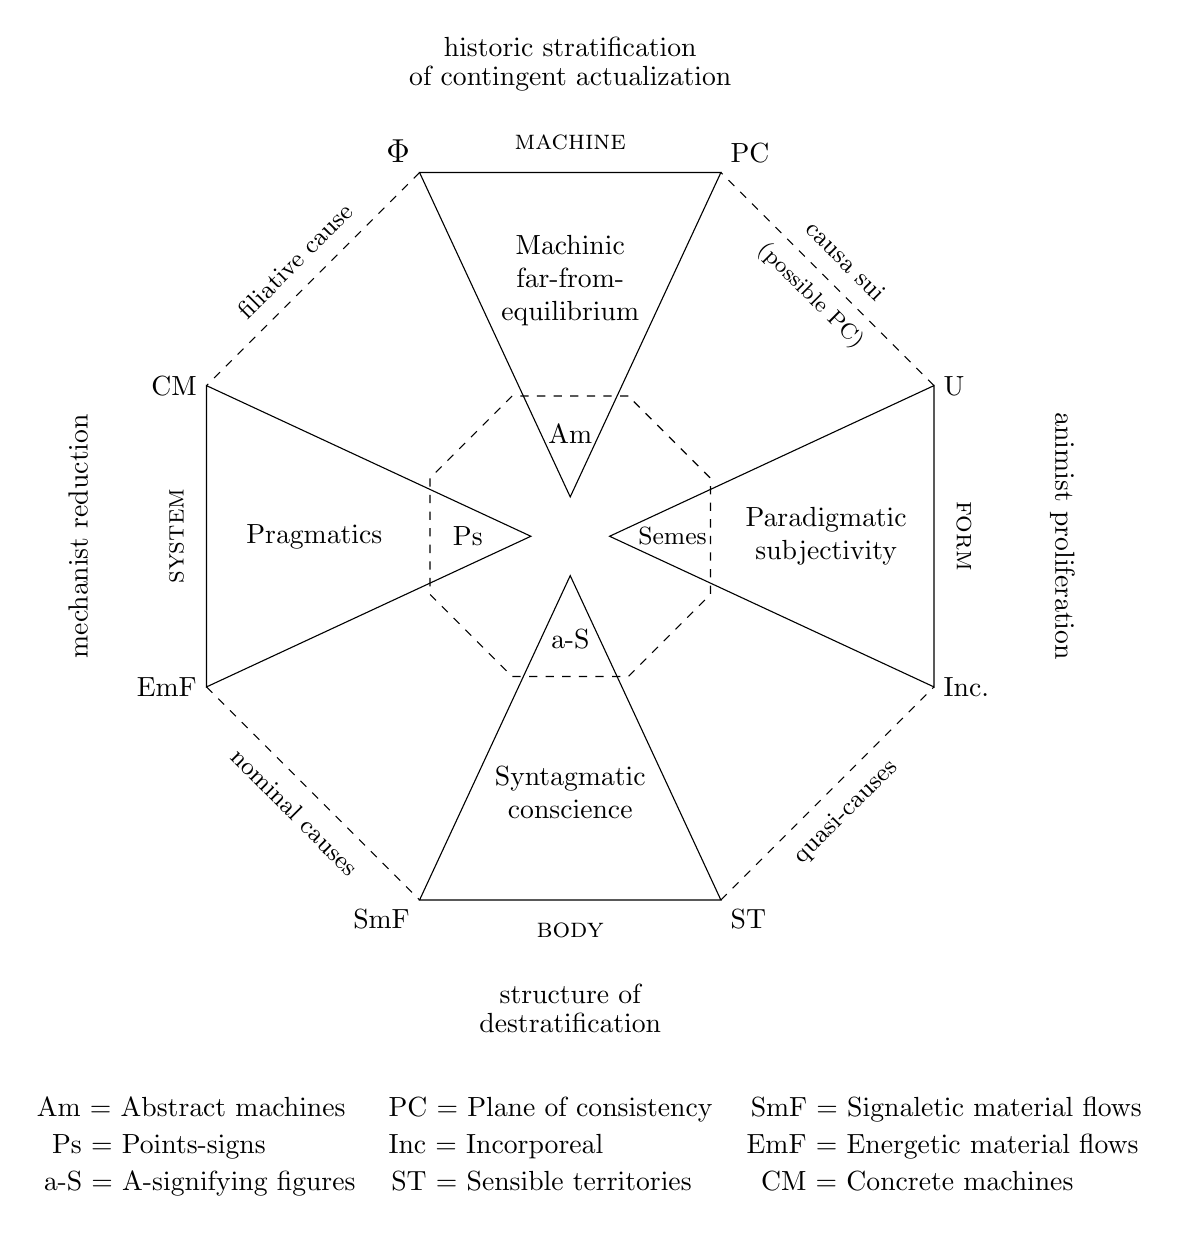
\begin{tikzpicture}	
	\def\s{5} %distance of octagon points from origin
	
	\foreach \i in {0,...,3}{
		\draw ({5*cos(\i*90-22.5)},{5*sin(\i*90-22.5)})--({0.5*cos(\i*90)},{0.5*sin(\i*90)})-- ({5*cos(\i*90+22.5)},{5*sin(\i*90+22.5)})--cycle;
		\draw[dashed] ({5*cos(\i*90+22.5)},{5*sin(\i*90+22.5)}) -- ({5*cos(\i*90+67.5)},{5*sin(\i*90+67.5)});
	}
	
	%INNER LABELS
	\node[regular polygon,regular polygon sides=8,draw,dashed,scale=10.75] {};
	\node at ({1.3*cos(0)},{1.3*sin(0)}) {\small Semes};
	\node at ({1.3*cos(90)},{1.3*sin(90)}) {Am};
	\node at ({1.3*cos(180)},{1.3*sin(180)}) {Ps};
	\node at ({1.3*cos(-90)},{1.3*sin(-90)}) {a-S};
	%													   %machinique loin de l'équilibre (?)
	\node[align=center] at ({3.25*cos(90)},{3.25*sin(90)}) {Machinic \\ far-from- \\ equilibrium};
	\node[align=center] at ({3.25*cos(0)},{3.25*sin(0)}) {Paradigmatic \\ subjectivity};
	\node[align=center] at ({3.25*cos(-90)},{3.25*sin(-90)}) {Syntagmatic \\ conscience};
	\node[align=center] at ({3.25*cos(180)},{3.25*sin(180)}) {Pragmatics};
	
	%OUTER LABELS
	\node at ( 0.7*\s, 0.7*\s) {\rotatebox{-45}{\small causa sui}};
	\node at ( 0.61*\s, 0.61*\s) {\rotatebox{-45}{\footnotesize (possible PC)}};
	\node at (-0.7*\s,-0.7*\s) {\rotatebox{-45}{\small nominal causes}};
	\node at (-0.7*\s, 0.7*\s) {\rotatebox{45}{\small filiative cause}};
	\node at ( 0.7*\s,-0.7*\s) {\rotatebox{45}{\small quasi-causes}};
	%
	\node at (0, \s) {\scshape machine};
	\node at (-\s,0) {\rotatebox{90}{\scshape system}};
	\node at ( \s,0) {\rotatebox{-90}{\scshape form}};
	\node at (0,-\s) {\scshape body};
	%
	\node[align=center] at (0,1.2*\s) {historic stratification \\[-0.5mm] of contingent actualization};
	\node[align=center] at (0,-1.2*\s) {structure of \\[-0.5mm] destratification};
	\node at ( 1.25*\s,0) {\rotatebox{-90}{animist proliferation}};
	\node at (-1.25*\s,0) {\rotatebox{90}{mechanist reduction}};
	%
	\node[above left] at ({\s*cos(90+22.5)},{\s*sin(90+22.5)}) {\large $\Phi$};
	\node[above right] at ({\s*cos(90-22.5)},{\s*sin(90-22.5)}) {PC}; 
	\node[right] at ({\s*cos(0+22.5)},{\s*sin(0+22.5)}) {U};
	\node[right] at ({\s*cos(0-22.5)},{\s*sin(0-22.5)}) {Inc.};
	\node[below right] at ({\s*cos(-90+22.5)},{\s*sin(-90+22.5)}) {ST};
	\node[below left] at ({\s*cos(-90-22.5)},{\s*sin(-90-22.5)}) {SmF};
	\node[left] at ({\s*cos(180+22.5)},{\s*sin(180+22.5)}) {EmF};
	\node[left] at ({\s*cos(180-22.5)},{\s*sin(180-22.5)}) {CM};
	
	%LEGEND
	\node[align=left,below] at (-4.75,-1.4*\s) {%
		Am = Abstract machines\\[0.5mm]
		\hspace{5.5pt}Ps = Points-signs\\[0.5mm]
		\hspace{2.5pt}a-S = A-signifying figures
	};
	\node[align=left,below] at (-0.25,-1.4*\s) {%
		PC = Plane of consistency\\[0.5mm]
		Inc = Incorporeal\\[0.5mm]
		\hspace{1pt}ST = Sensible territories
	};
	\node[align=left,below] at (4.75,-1.4*\s) {%
		\hspace{1.5pt}SmF = Signaletic material flows\\[0.5mm]
		EmF = Energetic material flows\\[0.5mm]
		\hspace{5.25pt}CM = Concrete machines
	};
	\end{tikzpicture}
	
\end{document}